\section{Instrumentos y Equipos}
\begin{itemize}
    \item Contactor electromagnético comercial (con datos de placa)
    \item Fuente de tensión alterna variable (Variac)
    \item Amperímetro (CA)
    \item Voltímetro (CA)
    \item Óhmetro
    \item Destornilladores y herramientas para desarme
    \item Cables de conexión
\end{itemize}

\section{Procedimiento de Laboratorio}

\subsection{Desarme y Análisis del Contactor}
\begin{enumerate}
    \item Desarmar el contactor cuidadosamente, identificando cada una de sus partes.
    \item Examinar la constitución física del circuito magnético: bobina, núcleo, armadura, contactos principales y auxiliares.
    \item Identificar las espiras de sombra y el entrehierro permanente.
    \item Responder las siguientes preguntas:
          \begin{enumerate}
              \item ¿Cuál es la función de las espiras de sombra?
              \item ¿Cuál es la función del entrehierro permanente?
              \item ¿Qué es la corriente de llamada y qué orden de magnitud tiene respecto a la corriente nominal?
              \item ¿Qué es la corriente de mantenimiento?
              \item ¿Qué es la tensión de mantenimiento?
          \end{enumerate}
    \item Rearmar el contactor.
\end{enumerate}

\subsection{Medición de Características Eléctricas}
\begin{enumerate}
    \item Medir la resistencia de la bobina con un óhmetro.
    \item Conectar el contactor a una fuente de tensión alterna variable a través del Variac, según el esquema de conexiones mostrado en la figura~\ref{fig:diagrama_conexiones}.
    
    \begin{figure}[htbp]
        \centering
        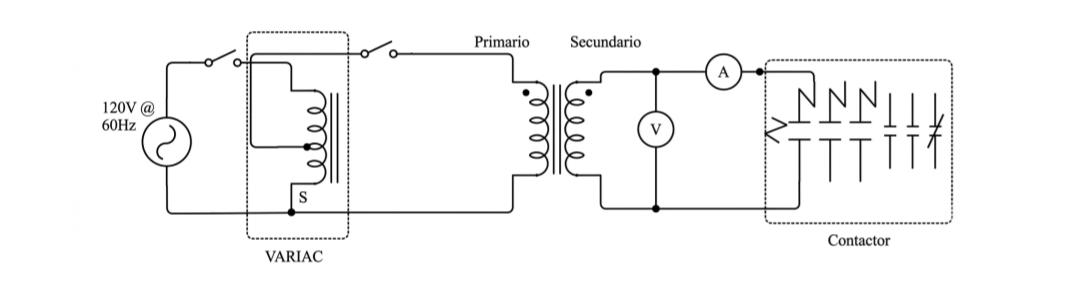
\includegraphics[width=0.7\textwidth]{figures/diagramas-de-conexiones-prelab3.jpeg}
        \caption{Diagrama de conexiones para la medición de características eléctricas del contactor.}
        \label{fig:diagrama_conexiones}
    \end{figure}

    \item Medir la corriente de llamada: alimentar el contactor impidiendo que cierre su circuito magnético (evitando que la armadura se desplace). Realizar la medición rápidamente, ya que la bobina no está diseñada para soportar esta corriente de forma permanente.
    \item Poner el contactor en posición normal de funcionamiento y medir:
          \begin{enumerate}
              \item Corriente de mantenimiento.
              \item Tensión de mantenimiento.
              \item Tensión mínima de operación (tensión a la cual el contactor comienza a cerrar).
          \end{enumerate}
    \item Comparar los resultados con la ficha técnica del contactor.
    \item Comentar si el contactor cumple con las características suministradas por el fabricante y qué significan funcionalmente estos parámetros.
\end{enumerate}
